\documentclass[12pt]{article}
\usepackage[latin1]{inputenc}
\usepackage[english]{babel}
\usepackage{amsmath}
\usepackage{amssymb}
\usepackage{dsfont}
\usepackage{theorem}
\usepackage{graphicx}
\usepackage{hyperref}
\usepackage{lscape}
\usepackage{enumerate}
\usepackage{verbatim}
\usepackage{float}
\usepackage{fancyhdr}
\usepackage{bigints}
\pagestyle{fancy}

\newtheorem{theorem}{Theorem}[section]
\newtheorem{lemma}[theorem]{Lemma}
\newtheorem{proposition}[theorem]{Proposition}
\newtheorem{corollary}[theorem]{Corollary}

\newenvironment{proof}[1][Proof:]{\begin{trivlist}
\item[\hskip \labelsep {\bfseries #1}]}{\end{trivlist}}
\newenvironment{definition}[1][Definition:]{\begin{trivlist}
\item[\hskip \labelsep {\bfseries #1}]}{\end{trivlist}}
\newenvironment{example}[1][Example:]{\begin{trivlist}
\item[\hskip \labelsep {\bfseries #1}]}{\end{trivlist}}
\newenvironment{remark}[1][Remark:]{\begin{trivlist}
\item[\hskip \labelsep {\bfseries #1}]}{\end{trivlist}}

\newcommand{\qed}{\nobreak \ifvmode \relax \else
      \ifdim\lastskip<1.5em \hskip-\lastskip
      \hskip1.5em plus0em minus0.5em \fi \nobreak
      \vrule height0.75em width0.5em depth0.25em\fi}

\newcommand*{\QEDA}{\hfill\ensuremath{\blacksquare}}
\newcommand*{\QEDB}{\hfill\ensuremath{\square}}

\newcommand{\dif}{\mbox{d}}

%---------------------------------
%\topmargin -.5 in
%\textheight 22 cm
%\textwidth 16 cm
%\oddsidemargin 0 cm
%\evensidemargin 0 cm
%---------------------------------


\title{Growing Degree Days - Project}
\author{A. Naveen, C. Chagas, A. Iyer, O. Abramov, E. Kielley, R. Brecht}
\date{\today}

\begin{document}

\maketitle
\vspace{5pt}
\tableofcontents
\vspace{40pt}

\section{Motivation}
We want to use Python and Bash scripts to analyse growing degree days for cities
in Canada. Growing degree days are used to predict when a flower or plant will 
bloom. 

\pagebreak
\section{Minimum core tasks}

\subsection{Files and Scripts}
\begin{description}
\item[gdd.sh]
\item Input: temperatures.csv, tbase, tupper
\item Output:
\item What it does... maybe adding code

\item[gdd.py]
\item Input: tbase, tupper
\item Output: year\_cityName\_gdd.csv
\item what it does...


\item[create\_plots.py]
\item Output: CumulativeGDD.png, CompareMaxMinTemp.png
\item Searches for all \emph{year\_cityName\_gdd.csv} files and generates a subplot for
each city. Then saves the generated plot into a PNG-file.
\end{description}
\subsection{Process flow}

\subsection{Results}
	\begin{figure}[!htbp]
		\centering
		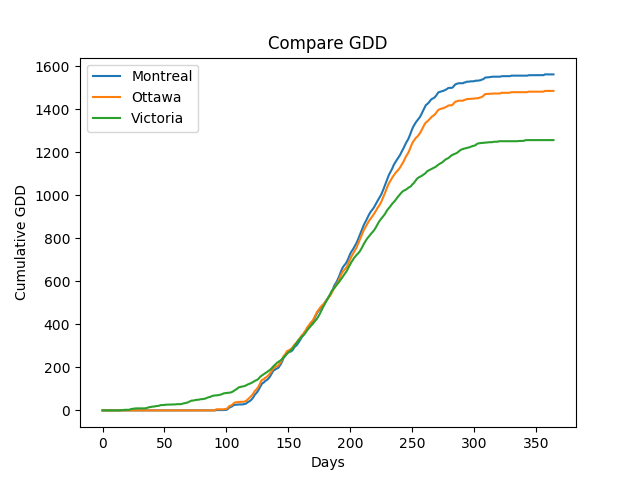
\includegraphics[width=0.9\textwidth]{./Plots/CumulativeGDD.png} 
		\caption{\scriptsize Shows the accumulated GDD vs time for three selected cities.}\label{GDDplot}		  
	\end{figure}

	\begin{figure}[!htbp]
		\centering
		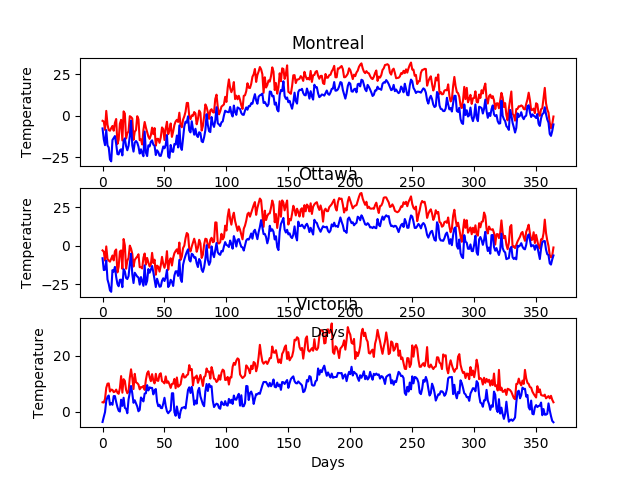
\includegraphics[width=0.9\textwidth]{./Plots/CompareMaxMinTemp.png} 
		\caption{\scriptsize Shows the min and max temperature for three selected cities.}\label{GDDplot}		  
	\end{figure}

\pagebreak
\section{Secondary tasks}


\end{document}
